% documentclass: article used for scientific journals, short reports, program documentation, etc
% options: fontsize 11, generate document for double sided printing, a4-paper
\documentclass[12pt, twoside, a4paper, fleqn]{article}

% package for changing page layout
\usepackage{geometry}
\geometry{a4paper, lmargin=40mm, rmargin=45mm, tmargin=40mm, bmargin=45mm}
% set indentation
\setlength{\parindent}{1em}
% set factor for line spacing
% \linespread{1.0}\selectfont
% set (dynamic) additional line spacing
% \setlength{\parskip}{1ex plus 0.5ex minus 0.3ex}

% rigorous formatting (not too much hyphens)
% \fussy
% \sloppy

% package for changing page layout (used to indent whole paragraphs with adjustwidth)
\usepackage{changepage}

% input encoding for special characters (e.g. ä,ü,ö,ß), only for non english text
% options: utf8 as encoding standard, latin1
\usepackage[utf8]{inputenc}
% package for font encoding
\usepackage[T1]{fontenc}
% package for changing used language (especially for more than one language)
% options: ngerman (new spelling) or default: english
\usepackage[ngerman]{babel}
% package for times font
% \usepackage{times}
% package for latin modern fonts
\usepackage{lmodern}

% package for math symbols, functions and environments from ams(american mathematical society)
\usepackage{amsmath}
\usepackage{mathtools}
% package for extended symbols from ams
\usepackage{amssymb}
% package for math black board symbols (e.g. R,Q,Z,...)
\usepackage{bbm}
% package used for calligraphic math symbols
\usepackage{mathrsfs}
% package for extended symbols from stmaryrd(st mary road)
\usepackage{stmaryrd}
% package for more math blackboard symbols
\usepackage{dsfont}

% pack­age im­ple­ments scal­ing of the math ex­ten­sion font cmex; used for scaling math signs
\usepackage{exscale}

% package for including extern graphics plus scaling and rotating
\usepackage{graphicx}
%package for positioning figures
\usepackage{float}
% package for changing color of font and paper
% options: using names of default colors (e.g red, black)
% \usepackage[usenames]{color}
\usepackage[dvipsnames]{xcolor}
\definecolor{shadecolor}{gray}{0.9}
% package for customising captions
\usepackage[footnotesize, hang]{caption}
% package for customising enumerations (e.g. axioms)
\usepackage{enumitem}
% calc package reimplements \setcounter, \addtocounter, \setlength and \addtolength: commands now accept an infix notation expression
\usepackage{calc}
% package for creating framed, shaded, or differently highlighted regions that can break across pages; environments: framed, oframed, shaded, shaded*, snugshade, snugshade*, leftbar, titled-frame
\usepackage{framed}
% package for creating custom "list of"
% options: titles: do not intefere with standard headings for "list of"
\usepackage[titles]{tocloft}
% change enumeration style of equations
% \renewcommand\theequation{\thesection.\arabic{equation}}


% provides \ifthenelse command
\usepackage{ifthen}
% extra commands for if-conditions (e.g. \isempty)
\usepackage{xifthen}

% init list of math for definitions and theorems
\newcommand{\listofmathcall}{Verzeichnis der Definitionen und Sätze}
\newlistof{math}{mathlist}{\listofmathcall}
% add parentheses around argument
\newcommand{\parent}[1]{ \ifx&#1&\else (#1) \fi }
\definecolor{mathdefback}{rgb}{0.95,0.95,0.98}
% unnumerated mathematical definition environment definiton
\newenvironment{mathdef*}[2]{
	\medskip
	\begin{tcolorbox}[colback=mathdefback, boxrule=0.5pt, colframe=black, boxsep=0pt, enhanced jigsaw, breakable, arc=3pt]
	\noindent
	{ \fontfamily{ppl}\selectfont \textbf{\textsc{#1:}} } ~ #2 
	\par \hfill\\ 
	\fontfamily{lmr}\selectfont \itshape
}{
	\end{tcolorbox}
	\medskip
}
% definitions for numerated mathematical definition environment
\newcounter{mathdefc}[section]
\newcommand*{\mathdefnum}{\thesection.\arabic{mathdefc}}
\renewcommand{\themathdefc}{\mathdefnum}
\newenvironment{mathdef}[2]{
	\refstepcounter{mathdefc}
	\addcontentsline{mathlist}{figure}{\protect{\numberline{\mathdefnum}#1 ~ #2}}
	\begin{mathdef*}{#1 \mathdefnum}{#2}
}{
	\end{mathdef*}
}
% standard mathdef calls
\newcommand{\definitioncall}{Definition}
\newenvironment{definition*}[1][]{ \begin{mathdef*}{\definitioncall}{\parent{#1}} }{ \end{mathdef*} }
\newenvironment{definition}[1][]{ \begin{mathdef}{\definitioncall}{\parent{#1}} }{ \end{mathdef} }

\definecolor{maththeoremframe}{rgb}{0.7,0.7,0.73}

% unnumerated theorem environment definition
\newenvironment{maththeorem*}[2]{
	\medskip
	\begin{tcolorbox}[boxrule=0pt, leftrule=2.5pt, arc=2pt, colback=white, colframe=maththeoremframe, enhanced jigsaw, breakable, vfill before first, top=0mm, bottom=0mm, left=2mm, right=0mm, boxsep=1mm]
	\noindent
	{ \fontfamily{ppl}\selectfont \textbf{\textsc{#1:}} } ~ #2
	\par \hfill\\ 
	\fontfamily{lmr} \fontshape{it} \selectfont
}{ 
	\end{tcolorbox}
	\medskip
}
% definitions for numerated theorem environment
\newcounter{maththeoremc}[section]
\newcommand*\maththeoremnum{\thesection.\arabic{maththeoremc}}
\renewcommand{\themaththeoremc}{\maththeoremnum}
\newenvironment{maththeorem}[2]{
	\refstepcounter{maththeoremc}
	\addcontentsline{mathlist}{figure}{\protect{\qquad\numberline{\maththeoremnum}#1 ~ #2}}
	\begin{maththeorem*}{#1 \maththeoremnum}{#2}
}{
	\end{maththeorem*}
}
% standard maththeorem calls
\newcommand{\theoremcall}{Theorem}
\newenvironment{theorem*}[1][]{ \begin{maththeorem*}{\theoremcall}{\parent{#1}} }{ \end{maththeorem*} }
\newenvironment{theorem}[1][]{ \begin{maththeorem}{\theoremcall}{\parent{#1}} }{ \end{maththeorem} }
\newcommand{\lemmacall}{Lemma}
\newenvironment{lemma*}[1][]{ \begin{maththeorem*}{\lemmacall}{\parent{#1}} }{ \end{maththeorem*} }
\newenvironment{lemma}[1][]{ \begin{maththeorem}{\lemmacall}{\parent{#1}} }{ \end{maththeorem} }
\newcommand{\propositioncall}{Proposition}
\newenvironment{proposition*}[1][]{ \begin{maththeorem*}{\propositioncall}{\parent{#1}} }{ \end{maththeorem*} }
\newenvironment{proposition}[1][]{ \begin{maththeorem}{\propositioncall}{\parent{#1}} }{ \end{maththeorem} }
\newcommand{\corollarycall}{Korollar}
\newenvironment{corollary*}[1][]{ \begin{maththeorem*}{\corollarycall}{\parent{#1}} }{ \end{maththeorem*} }
\newenvironment{corollary}[1][]{ \begin{maththeorem}{\corollarycall}{\parent{#1}} }{ \end{maththeorem} }
% q.e.d. definition
\newcommand{\qed}{ \par \hfill \fontfamily{lmr} \fontshape{it} \selectfont \mbox{q.e.d.} \\}
\newcommand{\qedbox}{ \hfill $\Box$ }
% proof environment definition for theorems
\newenvironment{mathproof}[2]{
	% \par\hfill\\
	\medskip
	% \noindent
	% \par
	% { \fontfamily{ppl}\selectfont \small \textsc{#1:} } ~ \parent{#2} \smallskip\\
	% \begin{adjustwidth}{1em}{}
	\begin{tcolorbox}[title= { \fontfamily{ppl}\selectfont \small \textsc{#1:} } ~ \parent{#2}, boxrule=0pt, colback=white, colframe=white, coltitle=black, breakable, boxsep=0mm, top=2mm, bottom=0mm, right=0mm, left=0mm, before upper={\parindent1em}]%
	\normalfont
	\small
}{ 
	\end{tcolorbox}
	% \end{adjustwidth} 
	% \qedbox
	\medskip
}
% standard mathproof calls
\newcommand{\proofcall}{Beweis}
\newenvironment{proof}[1][]{ \begin{mathproof}{\textbf{\proofcall}}{#1} }{ \qedbox \end{mathproof} }
\newcommand{\proofideacall}{Beweisidee}
\newenvironment{proofidea}[1][]{ \begin{mathproof}{\proofideacall}{#1} }{ \end{mathproof} }
\newcommand{\examplecall}{Beispiel}
\newenvironment{example}[1][]{ \begin{mathproof}{\examplecall}{#1} }{ \end{mathproof} }

% fast font types
\newcommand{\m}[1]{\mathrm{#1}}
\newcommand{\s}[1]{\mathcal{#1}}


% define
\newcommand{\define}{\coloneqq}
% define sign from the right
\newcommand{\definedby}{\eqqcolon}
% function
\newcommand{\func}[3]{#1\colon#2\to#3}


% brackets
% curly brackets
\newcommand{\curlb}[1]{\left\{ #1 \right\}}
% box brackets
\newcommand{\boxb}[1]{\left[ #1 \right]}
% parentheses/curved brackets
\newcommand{\curvb}[1]{\left( #1 \right)}
% angle brackets
\newcommand{\angleb}[1]{\left\langle #1 \right\rangle}
% floor brackets
\newcommand{\floorb}[1]{\left\lfloor #1 \right\rfloor}
% ceil brackets
\newcommand{\ceilb}[1]{\left\lceil #1 \right\rceil}


% symbols for sets
% create sets
% \newcommand{\set}[2][]{ \curlb{#2 \ifx&#1&\else \enspace\middle\vert\enspace #1 \fi} }
\newcommand{\set}[2][]{ \curlb{#2 \ifthenelse{\isempty{#1}}{}{\enspace\middle\vert\enspace #1}} }
% standard sets
\newcommand{\SR}{\mathds{R}} % real numbers
\newcommand{\SC}{\mathds{C}} % complex numbers
\newcommand{\SN}{\mathds{N}} % natural numbers
\newcommand{\SZ}{\mathds{Z}} % integral numbers
\newcommand{\SQ}{\mathds{Q}} % rational numbers
\newcommand{\SFP}{\mathds{P}} % polynom functions
\newcommand{\SFC}{\mathrm{C}} % complex valued functions (continous or differentiable)
\newcommand{\SFL}{\mathcal{L}} % space of integrable functions
\newcommand{\SFLL}{\mathrm{L}} % space of integrable function classes
% set of linear maps
\newcommand{\LM}{L}
% hilbert space
\newcommand{\SH}{\mathcal{H}}
% set of matrices
\newcommand{\SM}{\mathrm{M}}
% set of invertible
\newcommand{\SGL}{\mathrm{Gl}}
% group of orthogonal matrices
\newcommand{\SO}{\mathrm{O}}
% special group of orthogonal matrices
\newcommand{\SSO}{\mathrm{SO}}
% group of unitary matrices
\newcommand{\SU}{\mathrm{U}}
% hauptraum/generalized eigenspace
\newcommand{\hau}{\mathrm{Hau}}


% elements
% identity
\DeclareMathOperator{\id}{id}
% identity matrix
\newcommand{\idmat}{\mathrm{I}}
% normal distribution
\newcommand{\FN}{\mathcal{N}}


% operators
% inverse
\newcommand{\inv}[1]{ {#1}^{-1} }
% magnitude/absolute value
\newcommand{\abs}[1]{\left\vert #1 \right\vert}
% norm
\newcommand{\norm}[1]{\left\| #1 \right\|}
% power of set
\DeclareMathOperator{\setpow}{\mathcal{P}}
% real part
\DeclareMathOperator{\real}{Re}
% imaginary part
\DeclareMathOperator{\imag}{Im}
% complex conjugate
\newcommand{\conj}[1]{ \overline{#1} }
% diagonal matrix
\DeclareMathOperator{\diag}{diag}
% trace of matrix
\DeclareMathOperator{\tr}{tr}
% kernel of function
% \DeclareMathOperator{\ker}{ker}
% image of function
\DeclareMathOperator{\im}{im}
% annihilator
\DeclareMathOperator{\ann}{ann}
% transponent matrix
\newcommand{\transp}[1]{ {#1}^\m{T} }
% spectrum of matrix
\DeclareMathOperator{\spec}{\sigma}
% rank of matrix
\DeclareMathOperator{\rank}{rank}
% signum of permutation or number
\DeclareMathOperator{\sign}{sign}
% expectation
\DeclareMathOperator{\expect}{\mathbb{E}}
% variance
\DeclareMathOperator{\var}{var}
% fourier transform
\newcommand{\fourier}{\mathcal{F}}
% derivative
\DeclareMathOperator{\Deriv}{D}
\newcommand{\deriv}[1]{ {#1}^{\prime} }
\newcommand{\dderiv}[1]{ {#1}^{\prime\prime} }
\newcommand{\ddderiv}[1]{ {#1}^{\prime\prime\prime} }
\newcommand{\nderiv}[2][]{ \ifx&#1& \deriv{#2} \else {#2}^{(#1)} \fi }
\DeclareMathOperator{\pderiv}{\partial}
% infinitesimal difference
\newcommand{\diff}{\mathrm{d}}
% integral
\newcommand{\integral}[4]{\int_{#1}^{#2} #3\ \diff #4}
\newcommand{\Integral}[4]{\int\limits_{#1}^{#2} #3\ \diff #4}
\newcommand{\iintegral}[2]{\int #1\ \diff #2} % indefinite integral
% scalar product
\newcommand{\dotp}[1]{\angleb{#1}}
% cross product sign
\newcommand{\cross}{\times}
% sign for direct sum
\newcommand{\dsum}{\oplus}
% linear span
\newcommand{\lspan}[1]{\angleb{#1}}
% dual space
\newcommand{\dual}[1]{ {#1}^* }
\newcommand{\ddual}[1]{ {#1}^{**} }
% bra-vector
\newcommand{\ket}[1]{ \left| #1 \right\rangle }
% ket-vector
\newcommand{\bra}[1]{ \left\langle #1 \right| }
% bracket
\newcommand{\bracket}[2]{ \left\langle #1 \middle| #2 \right\rangle }
% expectation of operator
\newcommand{\opexpect}[1]{ \angleb{#1} }

% converges arrow
\newcommand{\conv}[1][]{\xrightarrow[]{#1}}


% append unit
\newcommand{\unit}[1]{\, \mathrm{#1}}



% package for init listings(non-formatted  text) e.g. different source codes
\usepackage{listings}


% definitions for listing colors
\definecolor{codeDarkGray}{gray}{0.2}
\definecolor{codeGray}{gray}{0.4}
\definecolor{codeLightGray}{rgb}{0.94,0.94,0.91}
\definecolor{codeBorder}{rgb}{0.34,0.24,0.21}
% predefinitions for listings
\newcommand{\listingcall}{Listing}
\newlength{\listingframemargin}
\setlength{\listingframemargin}{1em}
\newlength{\listingmargin}
\setlength{\listingmargin}{0.08\textwidth}
% \newlength{\listingwidth}
% \setlength{\listingwidth}{ ( \textwidth - \listingmargin * \real{2} + \listingframemargin * \real{2} ) }
% definitions for list of listings
\newcommand{\listoflistingscall}{\listingcall -Verzeichnis}
\newlistof{listings}{listinglist}{\listoflistingscall}
% style definition for standard code listings
\lstdefinestyle{std}{
	belowcaptionskip=0.5\baselineskip,
	breaklines=true,
	frameround=tttt,
	% frame=false,
	xleftmargin=0em,
	xrightmargin=0em,
	showstringspaces=false,
	showtabs=false,
	% tab=\smash{\rule[-.2\baselineskip]{.4pt}{\baselineskip}\kern.5em},
	basicstyle= \fontfamily{pcr}\selectfont\footnotesize\bfseries,
	keywordstyle= \bfseries\color{MidnightBlue}, %\color{codeDarkGray},
	commentstyle= \itshape\color{codeGray},
	identifierstyle=\color{codeDarkGray},
	stringstyle=\color{BurntOrange}, %\color{codeDarkGray},
	numberstyle=\tiny\ttfamily,
	% numbers=left,
	numbersep = 1em,
	% stepnumber = 1,
	% captionpos=t,
	tabsize=4,
	% backgroundcolor=\color{codebLightGray},
	rulecolor=\color{codeBorder},
	framexleftmargin=\listingframemargin,
	framexrightmargin=\listingframemargin
}
% definition for unnumerated listing
\newcommand{\inputlistingn}[3][]{
	\begin{center}
		\begin{adjustwidth}{\listingmargin}{\listingmargin}
			\centerline{ {\fontfamily{lmr}\selectfont \footnotesize \listingcall:}\quad {\footnotesize #2} }
			\lstinputlisting[style=std, #1]{#3}
		\end{adjustwidth}
	\end{center}
}
% definition for numerated listing
\newcounter{listingc}[section]
\newcommand*\listingnum{\thesection.\arabic{listingc}}
\renewcommand{\thelistingc}{\listingnum}
\newcommand{\inputlisting}[3][]{
	\refstepcounter{listingc}
	\addcontentsline{listinglist}{figure}{\protect{\numberline{\listingnum:} #2 } }
	% \inputlistingn[#1]{#2}{#3}
	\begin{center}
		\begin{adjustwidth}{\listingmargin}{\listingmargin}
			\centerline{ {\fontfamily{lmr}\selectfont \footnotesize \listingcall~\listingnum:}\quad {\footnotesize #2} }
			\lstinputlisting[style=std, #1]{#3}
		\end{adjustwidth}
	\end{center}
}


% package for including csv-tables from file
% \usepackage{csvsimple}
% package for creating, loading and manipulating databases
\usepackage{datatool}

% package for converting eps-files to pdf-files and then include them
\usepackage{epstopdf}
% use another program (ps2pdf) for converting
% !!! important: set shell_escape=1 in /etc/texmf/texmf.cnf (Linux/Ubuntu 12.04) for allowing to use other programs
% !!!			or use the command line with -shell-escape
% \epstopdfsetup{outdir=./}
% \epstopdfDeclareGraphicsRule{.eps}{pdf}{.pdf}{
% ps2pdf -dEPSCrop #1 \OutputFile
% }


% package for reference to last page (output number of last page)
\usepackage{lastpage}
% package for using header and footer
% options: automate terms of right and left marks
% \usepackage[automark]{scrpage2}
% \setlength{\headheight}{4\baselineskip}
% set style for footer and header
% \pagestyle{scrheadings}
% \pagestyle{headings}
% clear pagestyle for redefining
% \clearscrheadfoot
% set header and footer: use <xx>head/foot[]{Text} (i...inner, o...outer, c...center, o...odd, e...even, l...left, r...right)

% use that for mark to last page: \pageref{LastPage}
% set header separation line
% \setheadsepline[\textwidth]{0.5pt}
% set foot separation line
% \setfootsepline[\textwidth]{0.5pt}



\usepackage{tcolorbox}
% \usepackage{tikz}
% \tcbuselibrary{listings}
\tcbuselibrary{many}
\tcbset{fonttitle=\footnotesize}

\usepackage{array}

\allowdisplaybreaks

% \usepackage{epic, eepic}
\usepackage{epic}

\usepackage{natbib}
\bibliographystyle{plain}
\usepackage{url}

\usepackage{indentfirst}


\usepackage{titling}
\title{}
\author{}

\usepackage{fancyhdr}
\fancypagestyle{titlestyle}{
	\fancyhf{}
	% \fancyfoot[C]{\footnotesize\bigskip\thepage/\pageref{LastPage}}
	\fancyfoot{}
	\renewcommand{\footrulewidth}{0pt}
	\renewcommand{\headrulewidth}{0pt}
}

\fancypagestyle{mainstyle}{
	\fancyhf{}
	\fancyfoot[C]{\footnotesize\bigskip\thepage}
	\fancyhead[LO,RE]{\footnotesize \leftmark} %left
	\fancyhead[RO,LE]{\footnotesize} %right
	\renewcommand{\footrulewidth}{0.5pt}
	\renewcommand{\headrulewidth}{0.5pt}
}

\pagestyle{mainstyle}


\newcommand{\articletitle}{
	\thispagestyle{titlestyle}
	\hrule
	\section*{\centering \thetitle} % (fold)
	\noindent
	\parbox[b][][c]{0.5\textwidth}{\raggedright{\theauthor}}\hfill\parbox[b][][c]{0.5\textwidth}{\raggedleft{\email}}\\
	\hrule
	\bigskip
}


\DeclareMathOperator{\sign}{sign}

\AtBeginSection[]{
  \begin{frame}
  \vfill
  \centering
  \begin{beamercolorbox}[sep=8pt,center,shadow=true,rounded=true]{title}
  	\hrule
  	\bigskip
    \usebeamerfont{title}\insertsectionhead\par%
    \bigskip
    \hrule
  \end{beamercolorbox}
  \vfill
  \end{frame}
}

\begin{document}

	\begin{frame}
		\begin{figure}
			\centering
			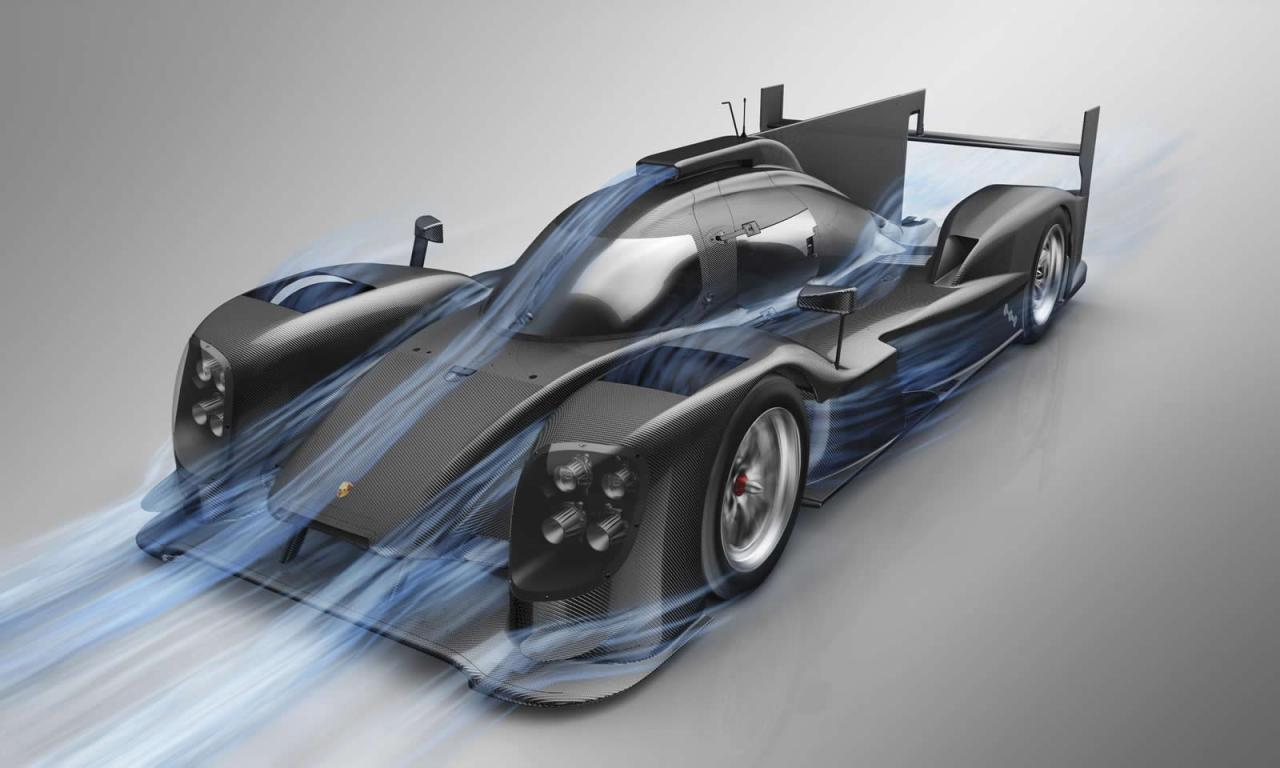
\includegraphics[scale=0.25]{images/Porsche-919-Hybrid-wind-tunnel-testing.jpg}
			\caption{Luftströmungen eines fahrenden Rennwagens \\ \scriptsize Quelle:\\ \url{http://autonetmagz.net/wp-content/uploads/2014/03/Porsche-919-Hybrid-wind-tunnel-testing.jpg}}
		\end{figure}
	\end{frame}
	
	\frame{\hrule\maketitle\hrule}
	\frame{\frametitle{Gliederung} \begin{adjustwidth}{1em}{}\tableofcontents\end{adjustwidth}}


	\section{Grundlagen} % (fold)
	\label{sec:grundlagen}

		\subsection{Erinnerung} % (fold)
		\label{sub:erinnerung}
		
			\begin{frame}
				\frametitle{Erinnerung: Thermodynamik}
				\begin{enumerate}[label=(\roman*)]
					\item Kontinuitätsgleichung:
						\[ \tcboxmath{\partial_t\varrho + \nabla\cdot\curvb{ \varrho\vec{v} } = 0} \]
					\item Impulsgleichung:
						\[ \tcboxmath{\varrho \boxb{ \partial_t \vec{v} + \curvb{ \vec{v}\cdot\nabla }\vec{v} } = \vec{f} + \nabla\cdot\sigma} \]
				\end{enumerate}
			\end{frame}
		
		% subsection erinnerung (end)


		\subsection{Navier-Stokes-Gleichungen} % (fold)
		\label{sub:navier_stokes_gleichungen}
		
			\begin{frame}
				\textbf{Annahme:}\\
				Betrachtung eines einzelnen newtonschen Fluids (z.B. Wasser, Öl, Luft, etc.).
				\vfill
				\pause
				\begin{tcolorbox}[title = Navier-Stokes Gleichungen]
					\begin{alignat*}{3}
						\partial_t\varrho + \nabla\cdot\curvb{ \varrho\vec{v} } &=&& \ 0 \\
						\varrho \boxb{ \partial_t \vec{v} + \curvb{ \vec{v}\cdot\nabla }\vec{v} } &=&& \ \vec{f} - \nabla p + \eta\Delta\vec{v} + \curvb{ \tfrac{\eta}{3}+\xi }\nabla\curvb{ \nabla\cdot\vec{v} }
					\end{alignat*}
				\end{tcolorbox}
			\end{frame}

			\begin{frame}[label=nsg]
				\begin{tcolorbox}[title = dimensionslose Navier-Stokes Gleichungen inkompressibler Flüssigkeiten]
					\begin{alignat*}{3}
						\nabla\cdot\vec{v} &=&& \ 0 \\
						\partial_t \vec{v} + \curvb{ \vec{v}\cdot\nabla }\vec{v} &=&& \ \vec{g} - \nabla p + \tfrac{1}{Re}\Delta\vec{v}
					\end{alignat*}
				\end{tcolorbox}
			\end{frame}
		
		% subsection navier_stokes_gleichungen (end)

	% section grundlagen (end)

	\section{Numerische Verfahren} % (fold)
	\label{sec:numerische_verfahren}
	
		\subsection{Diskretisierung} % (fold)
		\label{sub:diskretisierung}
		
			\begin{frame}
				\frametitle{Finite-Differenzen-Methode}
				\begin{enumerate}[label=(\roman*)]
					\item Vorwärts-Differenzenquotient
						\[ \tcboxmath{ u^\prime = \frac{u(x_{i+1}) - u(x_i)}{\delta x} + \mathcal{O}(\delta x) } \]
					\item Rückwärts-Differenzenquotient
						\[ \tcboxmath{ u^\prime = \frac{u(x_{i}) - u(x_{i-1})}{\delta x} + \mathcal{O}(\delta x) } \]
					\item zentraler Differenzenquotient
						\[ \tcboxmath{ u^\prime = \frac{u(x_{i+1}) - u(x_{i-1})}{2\delta x} + \mathcal{O}(\delta x^2) } \]
				\end{enumerate}
			\end{frame}

			\begin{frame}
				\frametitle{Verschobenes Gitter (staggered grid)}
				\begin{figure}
					\centering
					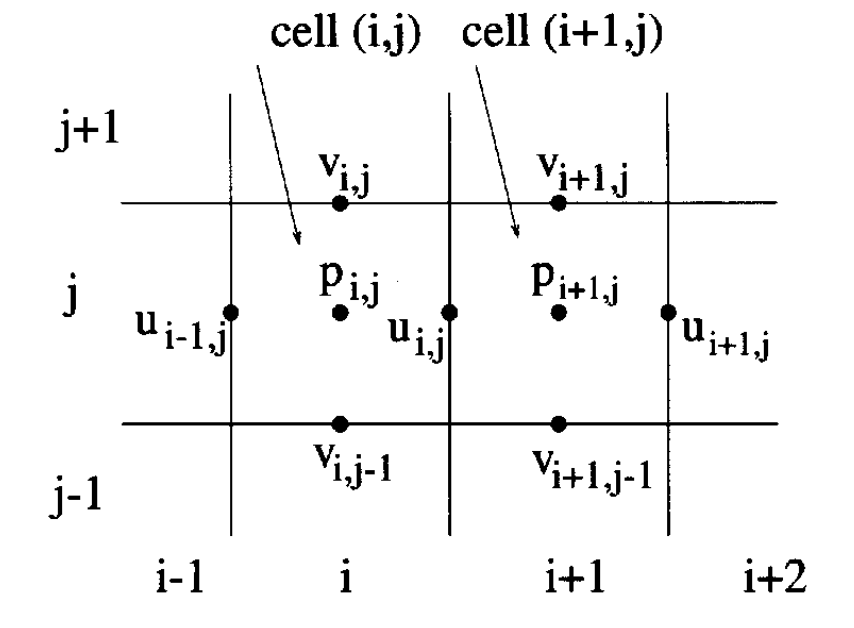
\includegraphics[scale = 0.30]{staggered-grid.png}
				\end{figure}
			\end{frame}

		% subsection diskretisierung (end)

		\subsection{Algorithmus} % (fold)
		\label{sub:algorithmus}
		
			\againframe{nsg}

		% subsection algorithmus (end)

	% section numerische_verfahren (end)

	\section{Ergebnisse} % (fold)
	\label{sec:ergebnisse}
	
		\begin{frame}
			\begin{figure}
				\centering
				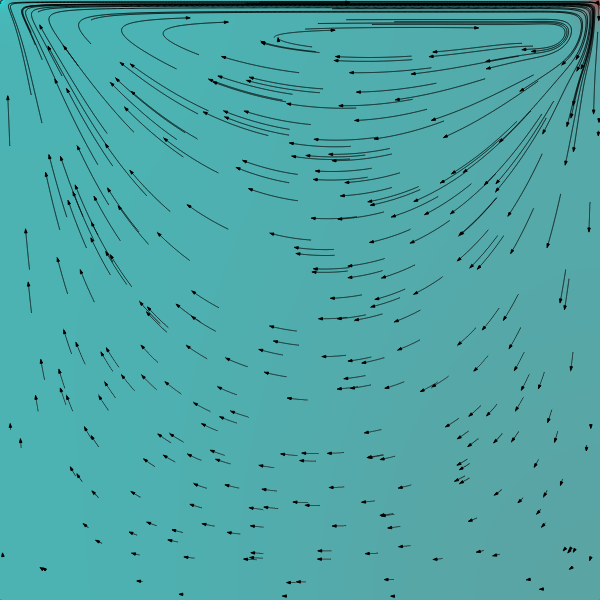
\includegraphics[scale=0.4]{images/re-1000-512-00520.png}
			\end{figure}
		\end{frame}

		\begin{frame}
			\begin{figure}
				\centering
				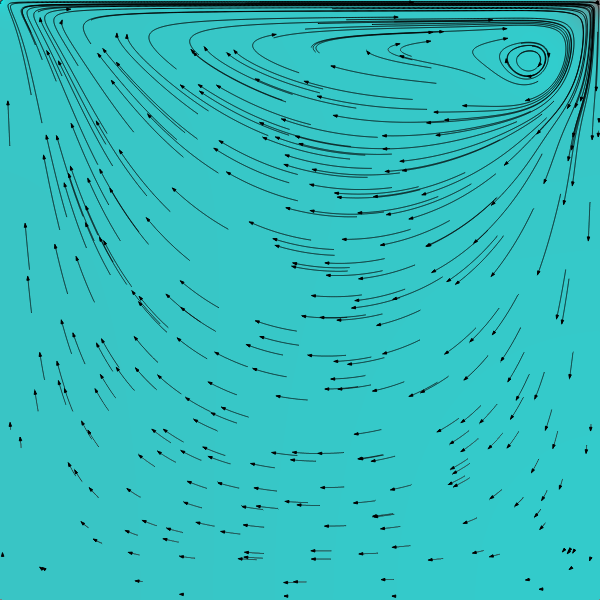
\includegraphics[scale=0.4]{images/re-1000-512-01069.png}
			\end{figure}
		\end{frame}

		\begin{frame}
			\begin{figure}
				\centering
				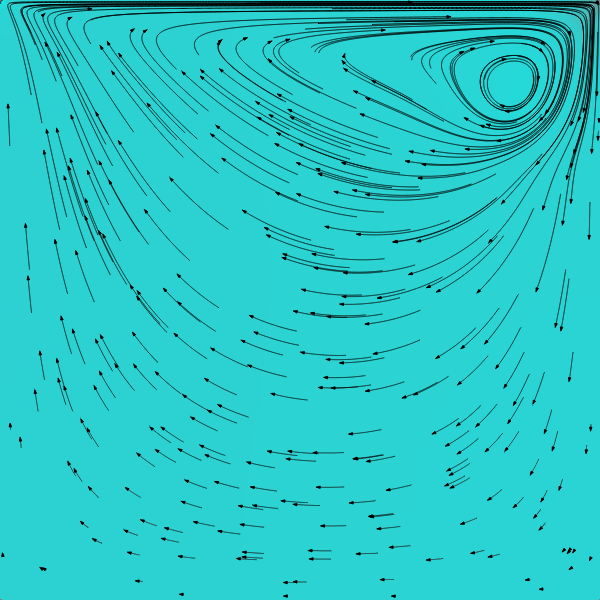
\includegraphics[scale=0.4]{images/re-1000-512-01555.png}
			\end{figure}
		\end{frame}

		\begin{frame}
			\begin{figure}
				\centering
				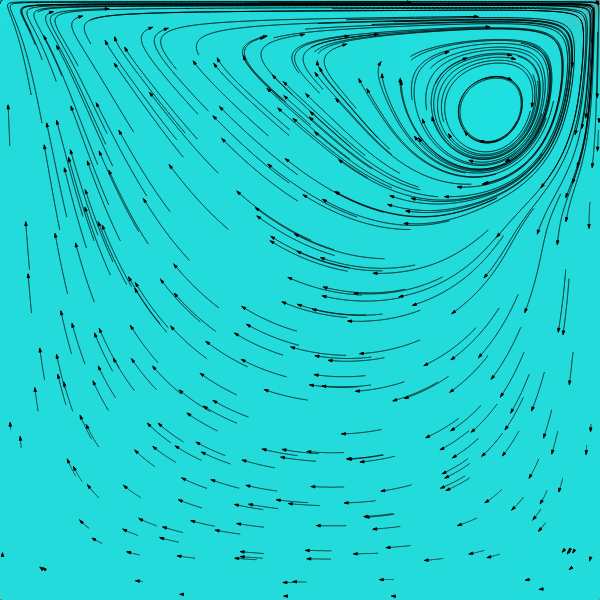
\includegraphics[scale=0.4]{images/re-1000-512-02170.png}
			\end{figure}
		\end{frame}

		\begin{frame}
			\begin{figure}
				\centering
				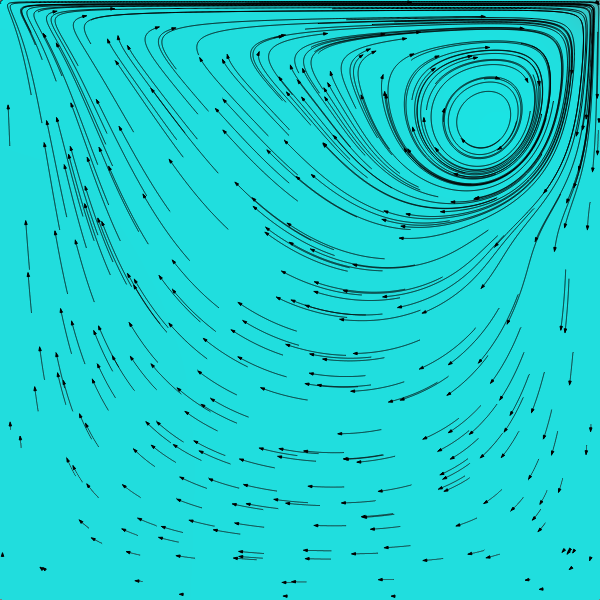
\includegraphics[scale=0.4]{images/re-1000-512-02405.png}
			\end{figure}
		\end{frame}

		\begin{frame}
			\begin{figure}
				\centering
				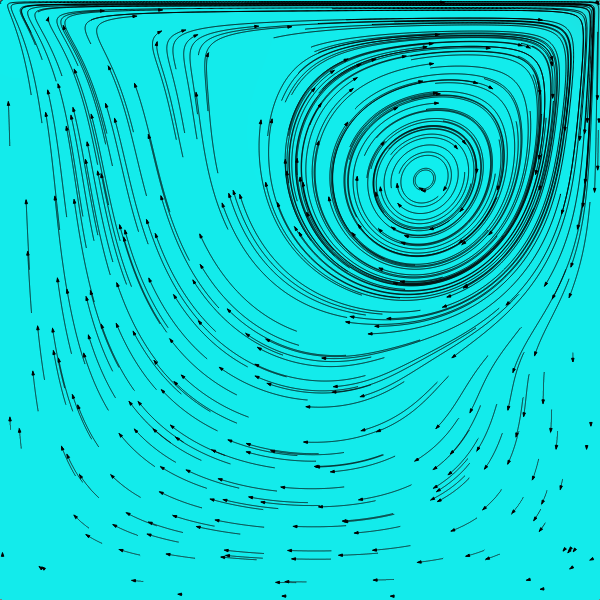
\includegraphics[scale=0.4]{images/re-1000-512-04758.png}
			\end{figure}
		\end{frame}

		\begin{frame}
			\begin{figure}
				\centering
				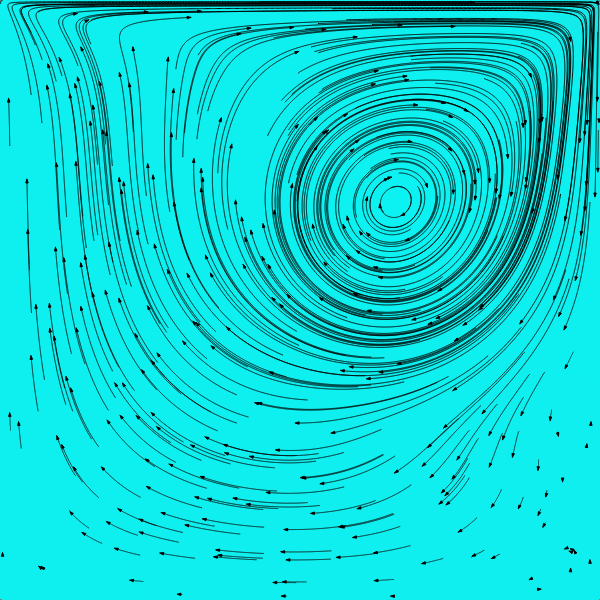
\includegraphics[scale=0.4]{images/re-1000-512-06482.png}
			\end{figure}
		\end{frame}

		\begin{frame}
			\begin{figure}
				\centering
				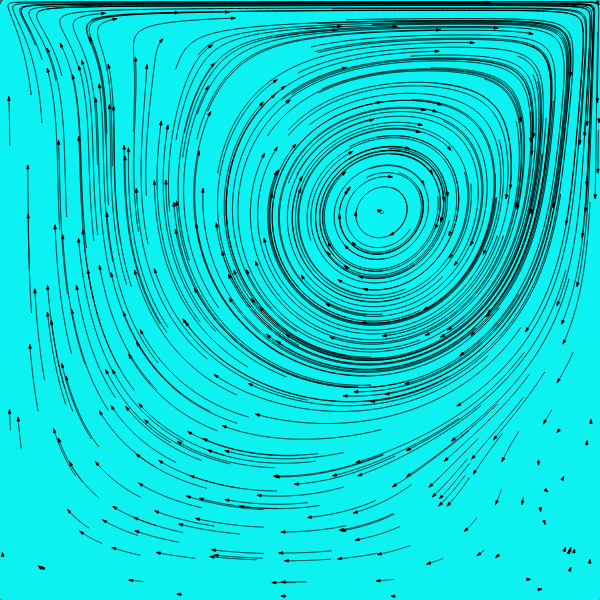
\includegraphics[scale=0.4]{images/re-1000-512-07612.png}
			\end{figure}
		\end{frame}

		\begin{frame}
			\begin{figure}
				\centering
				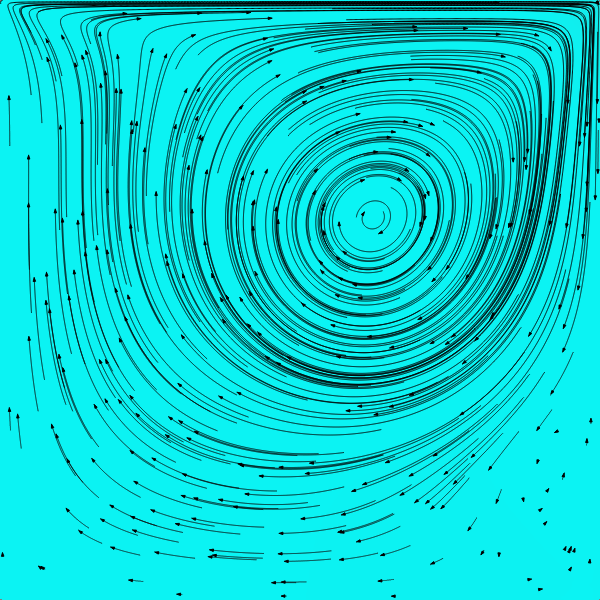
\includegraphics[scale=0.4]{images/re-1000-512-08419.png}
			\end{figure}
		\end{frame}

		\begin{frame}
			\begin{figure}
				\centering
				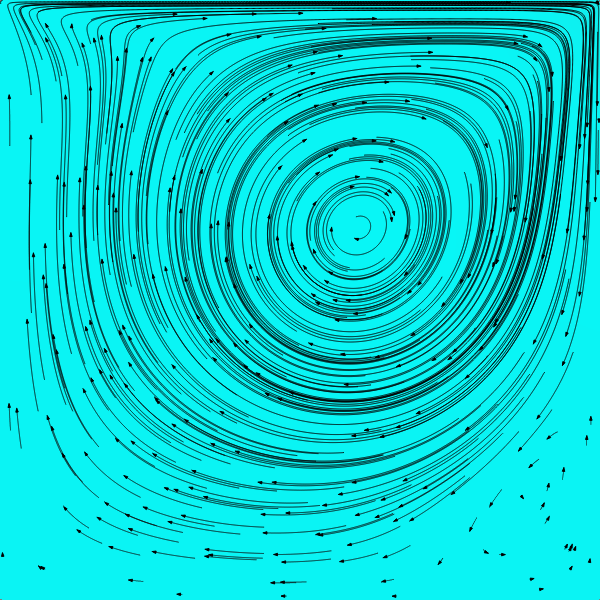
\includegraphics[scale=0.4]{images/re-1000-512-10164.png}
			\end{figure}
		\end{frame}

		\begin{frame}
			\begin{figure}
				\centering
				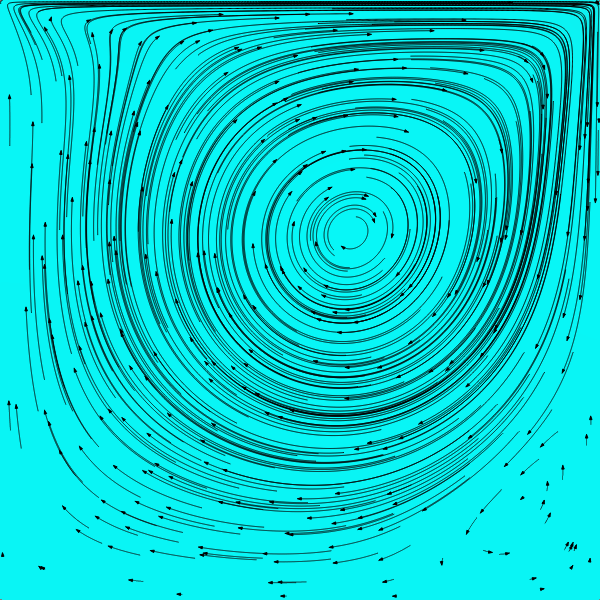
\includegraphics[scale=0.4]{images/re-1000-512-11408.png}
			\end{figure}
		\end{frame}

		\begin{frame}
			\begin{figure}
				\centering
				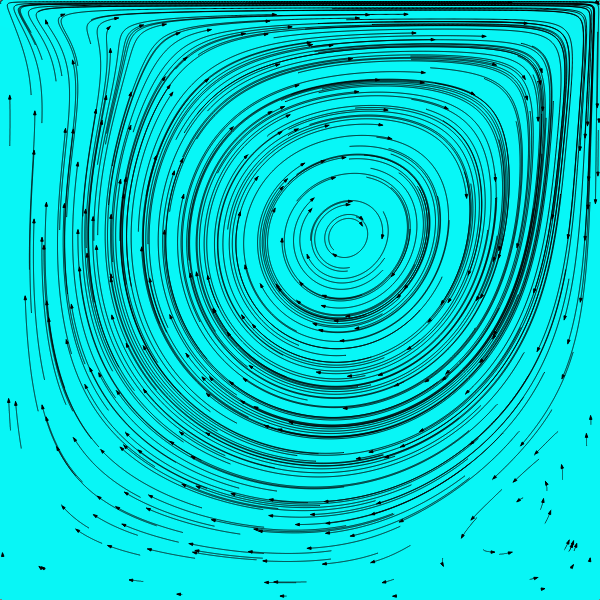
\includegraphics[scale=0.4]{images/re-1000-512-12475.png}
			\end{figure}
		\end{frame}

	% section ergebnisse (end)

	\section{Zusammenfassung} % (fold)
	\label{sec:zusammenfassung}

		\begin{frame}
			\textbf{grundsätzliches Verfahren:}
			\begin{itemize}[label=$\circ$]
				\item problemabhängige spezialisierte Navier-Stokes-Gleichungen
				\item Diskretisierung durch Gitter und Finite-Differenzen-Methode
				\item Aufstellen des linearen Gleichungssystems
				\item Lösen durch Zeitschrittverfahren und Poisson-Löser
				\item Anzeigen der Lösung
			\end{itemize}
		\end{frame}

		\begin{frame}
			\textbf{Probleme:}
			\begin{itemize}[label=$\circ$]
				\item numerische Instabilität für auftretende Turbulenzen
				\item viele numerische Verfahren sind problemabhängig
				\item sehr hoher Aufwand für komplexe Geometrien
				\item meistens nur qualitativer Vergleich mit Experimenten möglich
			\end{itemize}

			\begin{figure}
				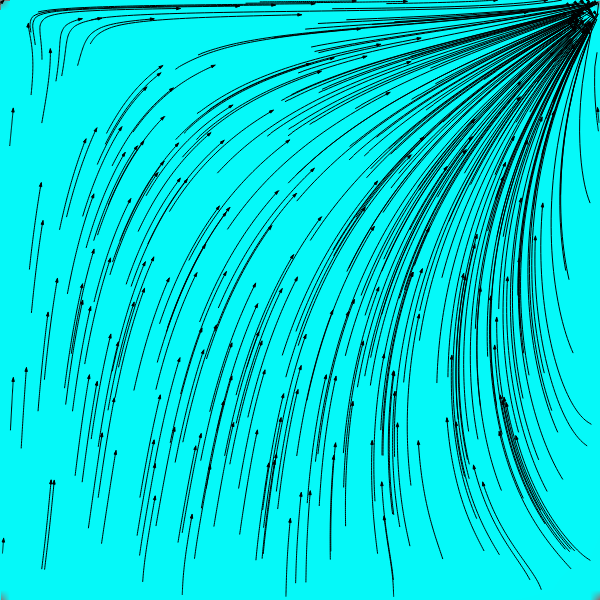
\includegraphics[scale = 0.2]{images/re-1000-64.png}
			\end{figure}
		\end{frame}

	% section zusammenfassung (end)
	
	\begin{frame}
		\frametitle{Referenzen}

		\begin{itemize}[label=$\circ$]
			\item Griebel und Dornseifer und Neunhoeffer, \textit{Numerical Simulation in Fluid Dynamics - A Practical Introduction}, 1998
			\item Ferziger und Peric, \textit{Computational Methods for Fluid Dynamics}, korrigierte 2.Auflage, 1997
			\item Durst, \textit{Grundlagen der Strömungsmechanik - Eine Einführung in die Theorie der Strömungen von Fluiden}, 2006
			\item Kincaid and Cheney, \textit{Numerical Analysis: Mathematics of Scientific Computing}, 3.Auflage, 2002
			\item Ansorg, Skript zu \textit{Thermodynamik und statistische Physik}, 2015/16
			\item \url{https://en.wikipedia.org/wiki/Computational_fluid_dynamics}
			\item \url{https://de.wikipedia.org/wiki/Navier-Stokes-Gleichungen}
		\end{itemize}
	\end{frame}

\end{document}